\documentclass[12pt]{article}

\usepackage[utf8]{inputenc}
\usepackage{amsmath}
\usepackage{fancyhdr}
\usepackage{graphicx}
\usepackage{vmargin}
\usepackage{chemfig}
\usepackage{tikz}
\usepackage{pgfplots}

%%%%%%%%%%%%%%%%%%%%%%%%%%%%%%%%%%%%%%%%%%%%%%%%%%%%%%%%%%%%%%%%%%%%%%%%%%

\setmarginsrb{3 cm}{2.5 cm}{3 cm}{2.5 cm}{1 cm}{1.5 cm}{1 cm}{1.5 cm}
\pagestyle{fancy}
\fancyhf{}
\rhead{2-5-2018}
\chead{Matematik aflevering 13}
\lhead{Jeppe Møldrup}
\rfoot{side \thepage}

%%%%%%%%%%%%%%%%%%%%%%%%%%%%%%%%%%%%%%%%%%%%%%%%%%%%%%%%%%%%%%%%%%%%%%%%%%

\begin{document}

\Large{\textbf{Matematik aflevering 13}}
\normalsize

\section*{Opgave 3.}
Jeg starter med bare at integrere min funktion $f(x)=4x^3-8x$
$$\int 4x^3-8x \ dx = x^4-\frac{8}{2}x^2+k$$
Så indsætter jeg mit punkt ind i funktionen og isolerer k
$$5=1^4-4 \cdot 1^2+k \leftrightarrow k=5-(1-4)=8$$
Så værdien for k hvis grafen skal skære i punktet $P(1,5)$ vil være $8$

\section*{Opgave 5.}
Tegn en mulig graf der opfylder at
$$f(0)=5 \ f(10)=-1$$
Og at fortegn og nulpunkter for $f'$ er som angivet på tallinien
\begin{center}
  \begin{tabular}{c c c c c c}
    x && 3 && 7 &\\
    \hline
    $f'(x)$ & - & 0 & + & 0 & -
  \end{tabular}
\end{center}

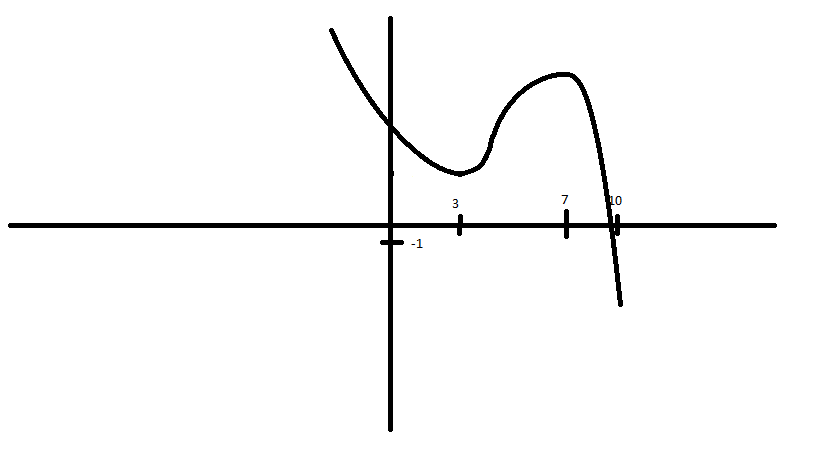
\includegraphics[width=\textwidth]{Graf1mat13.png}

\end{document}
